\documentclass{standalone}

\usepackage{tikz}
\usetikzlibrary{shapes.geometric, arrows, shadows, decorations.text}
\tikzstyle{startstop} = [rectangle, rounded corners, minimum width=3cm, minimum height=1cm,text centered, draw=black, fill=red!30, drop shadow]
\tikzstyle{io} = [trapezium, trapezium left angle=70, trapezium right angle=110, minimum width=3cm, minimum height=1cm, text centered, draw=black, fill=blue!30]
\tikzstyle{process} = [rectangle, minimum width=3cm, minimum height=1cm, text centered, text width=3cm, draw=black, fill=orange!30]
\tikzstyle{decision} = [diamond, minimum width=1cm, minimum height=1cm, text centered, draw=black, fill=green!30]
\tikzstyle{arrow} = [thick,->,>=stealth]
\tikzstyle{line} = [draw, -latex']

\begin{document}
  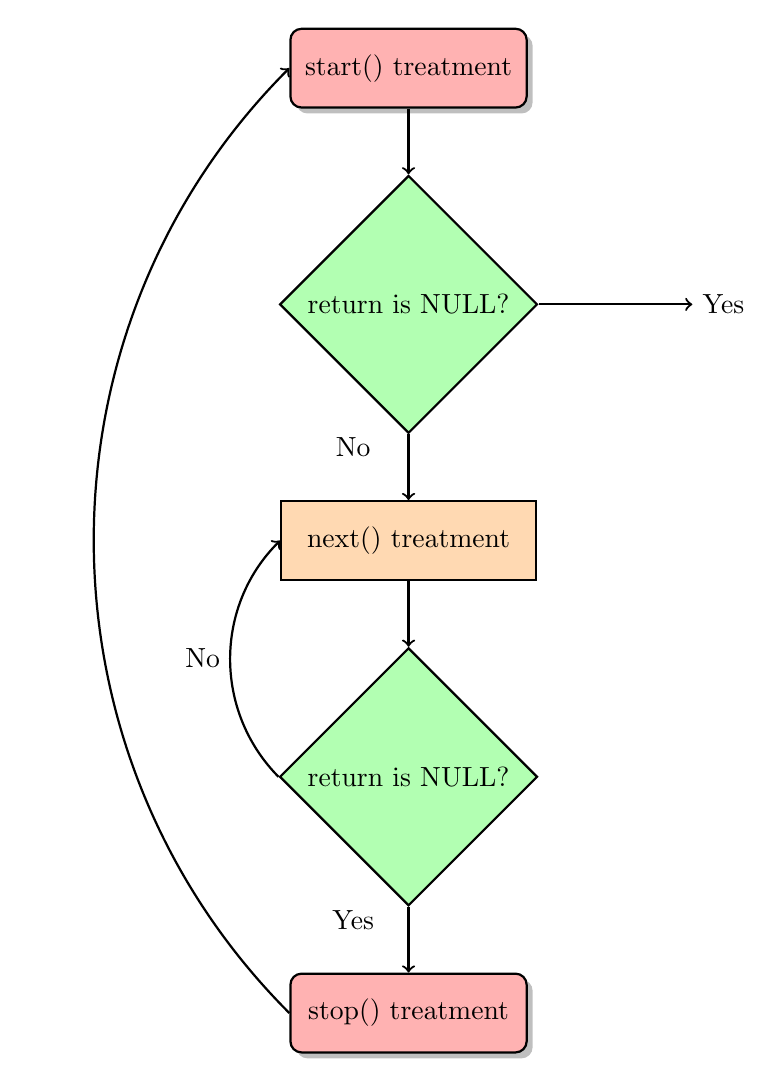
\begin{tikzpicture}[node distance=2cm, thick]
    \node (start) [startstop] {start() treatment};
    \node (branch1) [decision, below of=start, yshift=-1cm] {return is NULL?};
    \node (emptynode) [right of=branch1, xshift=2cm] {Yes};
    \node (next) [process, below of=branch1, yshift=-1cm] {next() treatment};
    \node (branch2) [decision, below of=next, yshift=-1cm] {return is NULL?};
    \node (stop) [startstop, below of=branch2, yshift=-1cm] {stop() treatment};

    \draw [->] (start) -- (branch1);
    \draw [->] (branch1) -- node[anchor=east] {} (emptynode);
    \draw [->] (branch1) -- node[left=2em, anchor=south] {No} (next);
    \draw [->] (next) -- (branch2);
    \draw [->] (branch2.west) to [out=135, in=-135, bend left=45] node [left] {No} (next.west);
    \draw [->] (branch2) -- node[left=2em, anchor=south] {Yes} (stop);
    \draw [->] (stop.west) to [out=135, in=-135] node [left] {} (start.west);
  \end{tikzpicture}
\end{document}
